\chapter{Vergelijking frameworks}
\label{ch:vergelijking-frameworks}
In dit hoofdstuk worden de opgezette frameworks met elkaar vergeleken op basis van het uitgevoerde experiment in overeenstemming met de requirements van Nubera. Beide frameworks worden uitvoerig behandeld en worden vergeleken op basis van dezelfde requirements. Dit hoofdstuk geeft de aanzet voor het vormen van een conclusie op de onderzoeksvraag en bijhorende deelonderzoeksvragen. De waarnemingen die in dit hoofdstuk aan bod komen werden allemaal waargenomen bij het opzetten van de Proof of Concept.

\section{Installatie framework}
\label{sec:vergelijking-installatie}
De installatie van OpenFaaS en Fission zijn gelijkaardig aan elkaar. Beide frameworks voorzien command line tools, voor het beheer ervan, die mee in de installatie zijn opgenomen. De stappen die doorlopen moeten worden voor het installeren van de frameworks zijn terug te vinden in de documentatie en kunnen eveneens worden geautomatiseerd. OpenFaaS beschikt over betere documentatie en how-to's die de installatie beschrijven. Het voordeel bij OpenFaaS is dat er standaard in de installatie reeds enkele features, zoals een user interface, aanwezig zijn. Bij installatie van Fission moet de UI nog apart worden toegevoegd. Gezien de standaard features die OpenFaaS meelevert bij installatie en de duidelijkere documentatie, neemt dit framework hier de voorkeur.

\section{Schrijven van functies}
De manier van functie deployment op beide frameworks verschilt en de vorm waarin de code moet worden geschreven is specifiek per framework. OpenFaaS bijvoorbeeld verwacht het gebruik van een ''handle'' methode die een request verwerkt als input parameter. Fission daarentegen verwacht het gebruik van een ''main'' methode zonder input parameters en gebruikt Flask voor het verwerken van HTTP requests. Functies moeten dus wel steeds worden aangepast aan het framework waarop ze draaien. Dit is jammer omdat op die manier geen generieke functies kunnen geschreven worden die op meerdere frameworks bruikbaar zijn, zo moeten functies vaak herschreven worden voor gebruik op een ander serverless framework. Beide benaderingen verschillen van elkaar en dat wat "best" is moet de ontwikkelaar zelf uitmaken. De frameworks bieden wel dezelfde functionaliteiten als het aankomt op schrijven van functies.

\section{Deployment van functies}
De manier waarop gebruikers functies kunnen deployen varieert tussen beide frameworks. Bij gebruik van OpenFaaS moet de gebruiker eerst voorgedefinieerde templates ophalen en deze aanvullen met de code om functionaliteit te voorzien. Vervolgens wordt er een Docker image gebuild en gepusht naar een Docker registry. Wanneer de image beschikbaar is in de registry, kan deze worden gebruikt om een de functie te deployen op het OpenFaaS framework. De volledige workflow kan worden uitgevoerd met de meegeleverde CLI tools die OpenFaaS aanbiedt. Functies kunnen ook via de UI worden gedeployed via OpenFaaS. Wanneer een functie wordt gedeployed, wordt er per functie een container opgezet waarin deze draait, dit is het standaardgedrag van OpenFaaS. OpenFaaS functies kunnen ook geconfigureerd worden zodat na verloop van tijd, als de functie lang geen requests ontvangt, de container wordt afgezet en weer ingeschakeld bij een nieuwe request. OpenFaaS voorziet de mogelijkheid om functies te definiëren in een YAML bestand en het framework leest hier alle waarden uit voor het deployen van een functie. Fission voorziet dit soort van functie templating met YAML bestanden niet.


Fission functie deployment werkt standaard op een andere manier. Indien een gebruiker een nieuwe functie wilt deployen dan moet deze eerst een environment aanmaken, specifiek voor de programmeertaal waarin de functie geschreven is. Vervolgens kan de gebruiker de functie deployen en de code (het bestand dat de code bevat met juiste extensie) meegeven zodat deze wordt gebruikt bij het uitvoeren van de functie. Na het deployen van een functie wordt er ook een route gedefinieerd zodat de functie kan worden aangeroepen via HTTP requests. Fission functies tonen een verschillend standaardgedrag ten opzichte van OpenFaaS. Wanneer een functie wordt gedeployed met default instellingen dan zal telkens wanneer deze wordt aangeroepen de code worden ingeladen in de environment containers en deze zullen de code uitvoeren. Om OpenFaaS en Fission op een gelijkaardige manier te vergelijken, werd het gedrag van OpenFaaS nagebootst. Fission laat toe om extra parameters te definiëren bij het deployen van functies, zo kan de gebruiker ervoor kiezen om het ''executortype'' aan te passen en ervoor te kiezen om de functie in een aparte container te draaien zoals aangehaald in sectie \ref{sec:fission-executors}. Het deployen van functies met een executortype van het type newdeploy komt overeen met de standaard deployment bij OpenFaaS.


Beide frameworks zijn erg gebruiksvriendelijk in het deployen van functies. Het voordeel bij Fission is dat het de mogelijkheid biedt om een route te creëren met een naam naar keuze voor het aanroepen van een functie. De route is een URL die wordt toegevoegd aan de Fission router en HTTP requests doorstuurt naar bijhorende functie. Het is ook interessant dat beide frameworks custom Docker containers toelaten die de gebruikers kunnen maken en gebruiken.
De deployment van functies is zeer specifiek, het is moeilijk een objectief oordeel te vellen over wat nu het beste zou zijn. Zoals eerder gezegd zijn beide frameworks erg gebruiksvriendelijk en is de deployment van functies een persoonlijk aspect afhankelijk van de gebruikers.

\section{Uitvoeringstijd van functies}
\label{sec:vergelijking-uitvoeringstijd}
Om inzicht te krijgen in het verschil in uitvoeringstijd van functies op beide frameworks werd de uitvoeringstijd van de zelfgeschreven Python demofunctie gemeten op beide frameworks. Daarnaast werd ook de uitvoeringstijd van een eenvoudige functie, nl. een ''Hello World'' functie, gemeten. De metingen uit bijlage \ref{sec:uitvoeringstijd-demofunctie} en bijlage \ref{sec:uitvoeringstijd-hello-world} worden vergeleken op basis van  berekeningen uitgevoerd in R. Onderstaande boxplots en tabellen geven inzicht in de metingen. De metingen werden uitgevoerd in een beheerste omgeving, nl. een Minikube cluster die eerder in dit onderzoek werd beschreven. De functies gedeployed op de frameworks draaien allen in een geïsoleerde container die specifiek voor één enkele functie wordt gebruikt, hierdoor worden cold starts vermeden en hoeft hier bij de data-analyse geen rekening gehouden worden. Daarnaast werden de metingen ook achtereenvolgens uitgevoerd, hierdoor kan aangenomen worden dat de datasets representatief zijn.

\newpage
\subsection{Uitvoeringstijd zelfgeschreven Python demofunctie}
De metingen op basis van dataset \ref{sec:uitvoeringstijd-demofunctie} geven inzicht in het verschil tussen uitvoeringstijd van de demofunctie op beide frameworks. Boxplot \ref{fig:boxplot-demo-functie} stelt de verwerkte gegevens visueel voor. De bekomen boxplot, centrum- en spreidingsmaten geven inzicht in het verschil tussen beide frameworks. Op  basis van de centrummaten is te zien dat de mediaan alsook het gemiddelde lager ligt bij Fission dan bij OpenFaaS, de demofunctie kent over het algemeen een iets kortere uitvoeringstijd bij Fission. Bij OpenFaaS zijn ook meer uitschieters terug te vinden maar dit is een factor waar niet op blindgestaard mag worden aangezien de functie gebruikmaakt van een API met authenticatie, deze kan mogelijks de uitschieters verklaren. Om een onderbouwd besluit te vorm wordt in volgende sectie de uitvoeringstijd van een simpele ''Hello World'' functie vergeleken, uitgevoerd op beide frameworks.
\begin{figure}
    \centering
    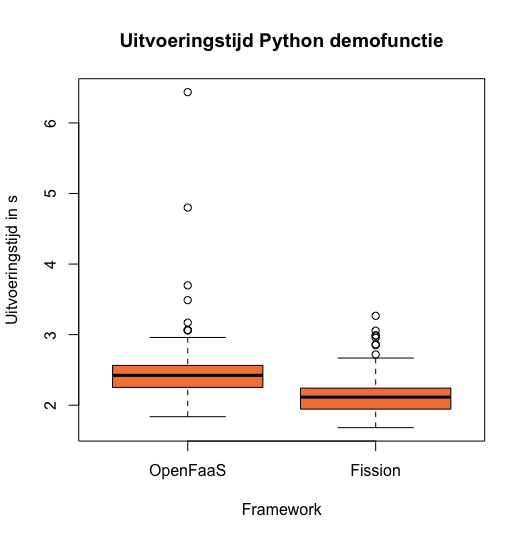
\includegraphics[width=0.6\textwidth]{img/boxplot-uitvoeringstijd-demofunctie.png}
    \caption{Boxplot uitvoeringstijd zelfgeschreven Python functie.}
    \label{fig:boxplot-demo-functie}
\end{figure}

\begin{tabular}{@{}lll@{}}
    \toprule
    & \textbf{OpenFaaS} & \textbf{Fission} \\ \midrule
    \textbf{Min.} & 1.837 & 1.682 \\
    \textbf{1st Qu.} & 2.253 & 1.946 \\
    \textbf{Median} & 2.423 & 2.114 \\
    \textbf{Mean} & 2.473 & 2.146 \\
    \textbf{3rd Qu.} & 2.564 & 2.242 \\
    \textbf{Max.} & 6.436 & 3.267 \\
    \textbf{Stdev.} & 0.423 & 0.267 \\ \bottomrule
\end{tabular}


\subsection{Uitvoeringstijd Hello World Python demofunctie}
De metingen op basis van dataset \ref{sec:uitvoeringstijd-hello-world} geven inzicht in het verschil tussen uitvoeringstijd van de eenvoudige ''Hello World'' functie op beide frameworks. Boxplot \ref{fig:boxplot-hello-functie} stelt de verwerkte gegevens visueel voor.
De boxplot die bekomen wordt door het vergelijken van de uitvoeringstijd, de spreidings- en centrummaten geven inzicht in het verschil tussen beide frameworks. Bij het evalueren van de centrummaten is alweer te zien dat het gemiddelde en de mediaan hoger ligt bij OpenFaas dan bij Fission. De standaardafwijking daarentegen ligt lager bij OpenFaas waardoor uitvoeringstijd constanter is dan bij Fission. De concentratie van de data bij Fission ligt veel dichter bij de mediaan ten opzichte van de data bij OpenFaaS.
\begin{figure}
    \centering
    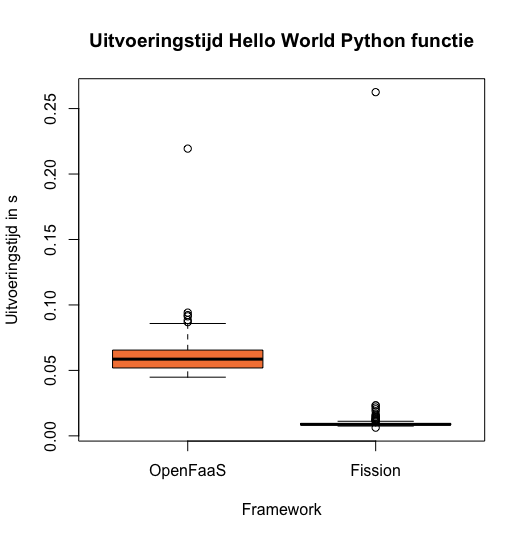
\includegraphics[width=0.6\textwidth]{img/boxplot-uitvoeringstijd-hellofunctie.png}
    \caption{Boxplot uitvoeringstijd Hello World Python functie.}
    \label{fig:boxplot-hello-functie}
\end{figure}

\begin{tabular}{@{}lll@{}}
    \toprule
    & \textbf{OpenFaaS} & \textbf{Fission} \\ \midrule
    \textbf{Min.} & 0.04482 & 0.00626 \\
    \textbf{1st Qu.} & 0.05190 & 0.00832 \\
    \textbf{Median} & 0.05860 & 0.00877 \\
    \textbf{Mean} & 0.06080 & 0.01061 \\
    \textbf{3rd Qu.} & 0.06541 & 0.00945 \\
    \textbf{Max.} & 0.21941 & 0.26255 \\
    \textbf{Stdev.} & 0.01518 & 0.01806 \\ \bottomrule
\end{tabular}

\subsection{Conclusie uitvoeringstijd}
Op basis van voorgaande berekeningen en boxplots is het duidelijk dat het Fission framework een snellere uitvoeringstijd van functies voorziet. Het verschil in uitvoeringstijd bij de zelfgeschreven Python functie valt echter relatief goed mee, het verschil bij de simpele ''Hello World'' functie is aanzienlijk groter. Het verschil lijkt in de opgestelde boxplots vrij groot maar in realiteit is dit echter nauwelijks merkbaar en zorgt dit niet voor grote hinder bij gebruikers. De verschillen in uitvoeringstijd is mogelijks te verklaren doordat beide frameworks gebruikmaken van voorbereide custom containers voor het uitvoeren van functies die door de medewerkers van het project werden gecreëerd. Het kan zijn dat de OpenFaaS container zwaarder is en meer processen draait waardoor de code iets trager uitgevoerd kan worden. De uitvoeringstijd is echter geen doorslaggevende factor voor het kiezen van een interessant framework. Doch kan deze factor in acht worden genomen bij het kiezen van een framework voor applicaties die continue de functies aanspreken en heel snel requests moeten bolwerken.

\section{Gebruik van de frameworks}
\subsection{Documentatie}
De frameworks beschikken beide over een mooie website waarop de documentatie op een duidelijke manier wordt gerepresenteerd. Op het eerste zin ziet de documentatie bij de frameworks er zeer compleet en duidelijk uit maar dit is echter te betwisten. De documentatie over OpenFaaS zat erg goed in elkaar met duidelijke voorbeelden en up-to-date code voor het opzetten van de omgeving als voor het deployen en het beheer van functies. Naast de documentatiewebsite zijn er ook veel bronnen over OpenFaaS terug te vinden zoals demo's of talks op conferenties. De documentatie van Fission daarentegen is beduidend minder kwaliteitsvol dan die van OpenFaaS. Fission beschikt in eerste instantie over relatief weinig documentatie, wat het voor beginners moeilijk maakt om hiermee aan de slag te gaan. De manier waarop bepaalde zaken in Fission werken zijn niet heel duidelijk beschreven in de documentatie en overigens zijn er ook weinig extra bronnen over terug te vinden. OpenFaaS biedt op dit moment de beste en meest duidelijke documentatie aan gebaseerd op eigen mening.

\subsection{User interface}
OpenFaaS voorziet standaard in de installatie een user interface. Gebruikers kunnen via de UI functies deployen en beheren. De instap, voor gebruikers zonder ervaring met FaaS frameworks en functies, is zeer laagdrempelig gezien de duidelijke en eenvoudige UI. Via de interface is het eenvoudig om demofuncties te deployen en deze ook te testen. Bij Fission daarentegen moest de UI na installatie van het framework nog bijkomstig worden geïnstalleerd. De UI van Fission is een ''early alpha'' versie die zelfs niet verenigbaar is met de Fission versie die in dit onderzoek werd gebruikt. De UI kon worden geraadpleegd maar geen enkele functionaliteit ervan bleek te werken. OpenFaaS is duidelijk een winnaar op basis van de huidige user interfaces.

\subsection{Command line tools}
Beide frameworks bieden CLI tools voor het beheer van de infrastructuur. De tools zijn beiden erg gebruiksvriendelijk en voorzien eveneens een duidelijke help functie met uitleg over de commando's. De volledige frameworks zijn te beheren via de command line, dit zorgt ervoor dat zaken makkelijk te reproduceren zijn. De enige bemerking bij dit onderdeel is dat Fission geen ''brew'' package heeft voor het installeren van de Fission CLI tools op macOS in tegenstelling tot OpenFaaS.

\subsection{Monitoring}
Fission en OpenFaaS voorzien standaard Prometheus voor het verzamelen van metrics en monitoring van de omgeving. Beide ondersteunen additionele dashboards die achteraf bovenop Prometheus kunnen worden geïnstalleerd voor het visueel representeren van metrics die werden verzameld. De frameworks scoren allebei goed op dit onderdeel, FIssion voorziet standaard ook Istio voor het management van de services en containers.

\section{Schaalbaarheid functies}
OpenFaaS en Fission schalen functies als de load verhoogd of verlaagd. Wanneer het CPU verbruik van een functiecontainer boven een zekere limiet gaat worden er extra functiecontainers opgezet en worden requests naar functies verdeeld door load-balancing. Vooraleer dit in werking treedt bij Fission moet het executortype worden ingesteld bij deployment van de functie, dit werd al uitvoerig in sectie \ref{sec:fission-executors} behandeld. In de Proof of Concept werd er een demo gegeven waarin functie autoscaling werd getriggerd in het geval van OpenFaaS. De demo gaf mooi weer dat er effectief extra containers werden opgezet als de load verhoogde. De demo van Fission daarentegen was eerder teleurstellend omdat autoscaling niet kon gedemonstreerd worden door onderliggende problemen. Volgens experten zijn de problemen te wijten aan onderliggende componenten, nl. metrics-server voor het verzamelen van metrics omtrent CPU en dergelijke. Beide frameworks voorzien effectief autoscaling desondanks dat dit niet bij allebei kon worden gedemonstreerd. Er wordt vanuit gegaan dat, in een productieomgeving die bestaat uit een Kubernetes cluster met meerdere nodes, de functies autoscalen indien de load hoger wordt. De OpenFaaS demo gaf wel een knap voorbeeld van hoe snel en effectief de autoscaling in zijn werk gaat. Autoscaling biedt een groot voordeel in het beheer van resources, er worden meer recources verbruikt bij veel requests maar wanneer er weer minder requests zijn worden er bijgevolg ook minder resources verbruikt. Het beste framework in dit onderdeel kan moeilijk worden gekozen wegens de mislukte demo. Indien beiden werkten zoals het zou moeten dan blijkt Fission eenvoudiger in het definiëren van additionele parameters voor het instellen van autoscaling. Bij gebruik van Fission is het mogelijk het minimum en maximum aantal pods te definiëren bij het deployen van functies.